\section{Introdução}

\begin{frame}\frametitle{Introdução}

Programas que usam E/S não-bloqueantes tendem a seguir a regra que toda
função deve retornar imediatamente.

\begin{quote}
Isso parece uma \emph{thread} não?

\end{quote}
Existem diferenças. Vejamos um exemplo da vida real.

\end{frame}

\begin{frame}\frametitle{Recepcionista do médico}

\framesubtitle{Doutor é quem tem doutorado}

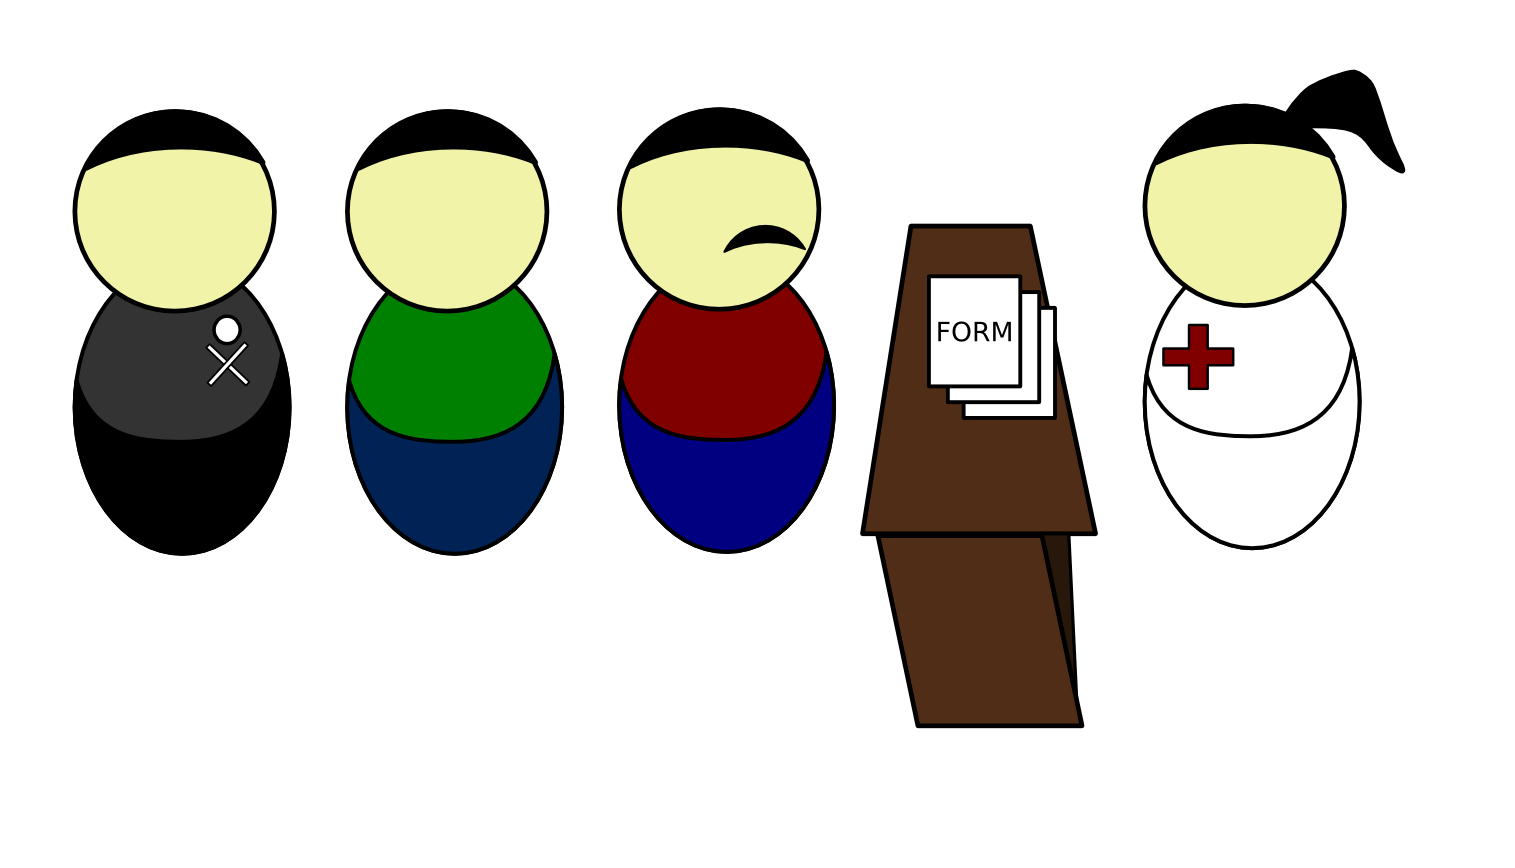
\includegraphics[scale=0.35]{img/ex1-1.png}

Imaginem uma fila na recepção de um consultório médico.

\end{frame}

\begin{frame}\frametitle{Recepcionista do médico}

\framesubtitle{Doutor é quem tem doutorado}

Para ser atendido o paciente precisa preencher \textbf{3 formulários}.

Num mundo bloqueante o paciente preencheria os \textbf{3 formulários} na
própria recepção, fazendo com que a fila espere.

Usando outra \emph{thread} (recepcionista) poderíamos resolver este
problema?

\end{frame}

\begin{frame}\frametitle{Recepcionista do médico}

\framesubtitle{Doutor é quem tem doutorado}

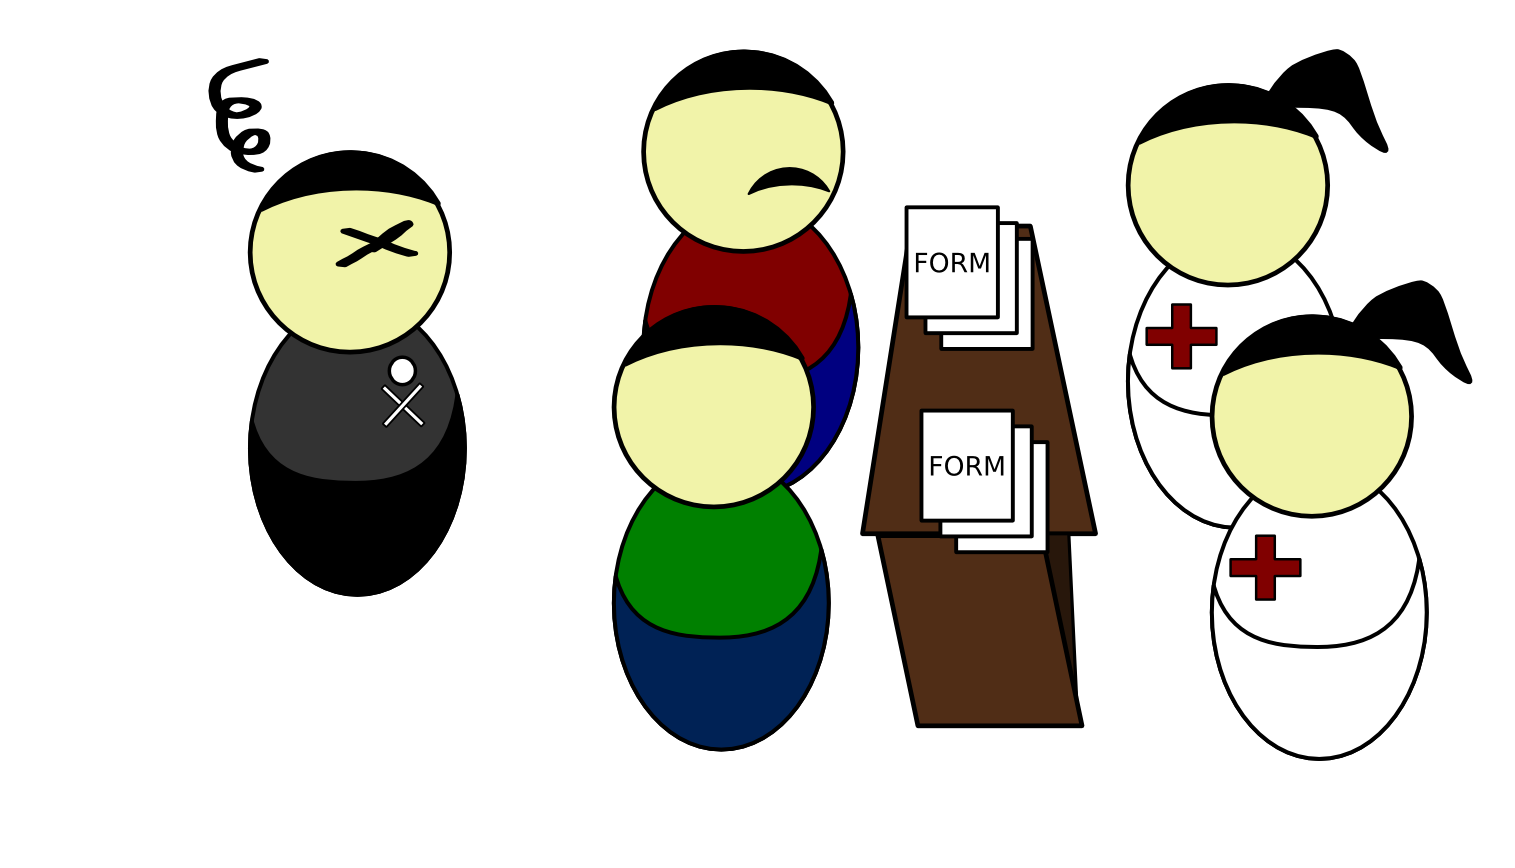
\includegraphics[scale=0.35]{img/ex1-2.png}

Parcialmente, já que mesmo assim a fila deve esperar. Mas como fazer com
que a fila não precise esperar?

\end{frame}

\begin{frame}\frametitle{Recepcionista do médico}

\framesubtitle{Doutor é quem tem doutorado}

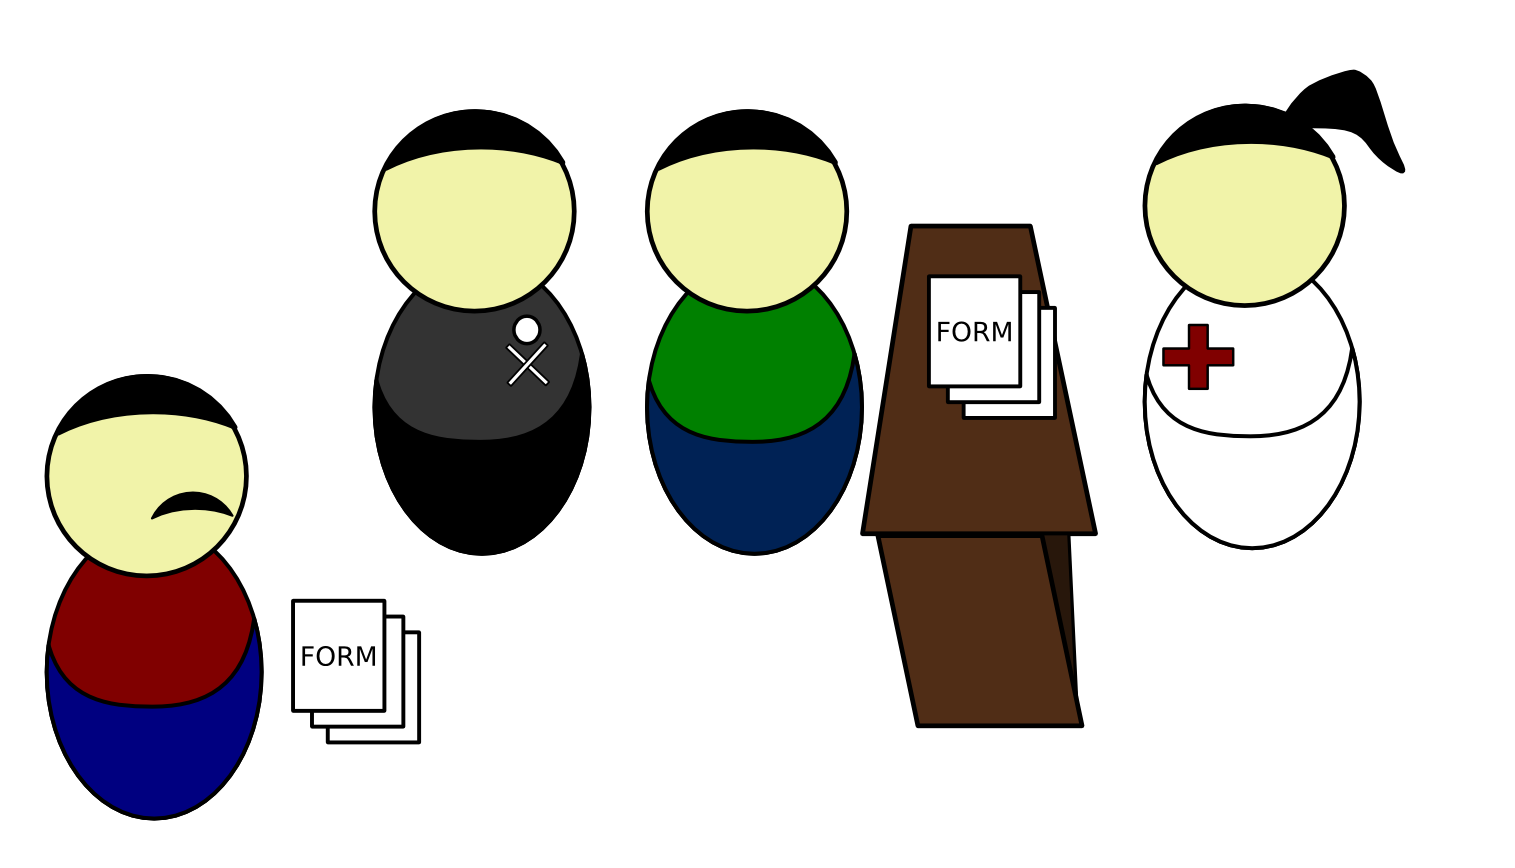
\includegraphics[scale=0.35]{img/ex1-3.png}

Enquanto um preenche o formulário, o outro é antendido. E assim por
diante. Dessa forma quando um paciente termina de preencher ele volta a
fila apenas para entregar o formulário e ser atendido em seguida.

\end{frame}

\section{NodeJS}

\begin{frame}\frametitle{NodeJS}

Uma das formas de implementarmos esse comportamento em uma linguagem de
programação é usando \href{http://nodejs.org/}{NodeJS}. Rodando em cima
do ambiente V8 do Google Chrome, NodeJS consegue trabalhar fora do
browser usando JavaScript.

\end{frame}

\begin{frame}[fragile]\frametitle{Hello World}

Instalação: \texttt{\$ sudo apt-get install nodejs}

\inputjscodefile{ src/hello.js }

Salve como \texttt{hello.js}. Execute num terminal:

\begin{verbatim}
$ node hello.js
\end{verbatim}
\end{frame}

\section{Emitindo eventos}

\begin{frame}\frametitle{Emitindo eventos}

\inputjscodefile{ src/event-emitter-1.js }

\end{frame}

\begin{frame}\frametitle{Emitindo eventos}

\inputjscodefile{ src/event-emitter-2.js }

\end{frame}

\begin{frame}\frametitle{Emitindo eventos}

\inputjscodefile{ src/event-emitter-3.js }

\end{frame}

\begin{frame}\frametitle{Emitindo eventos}

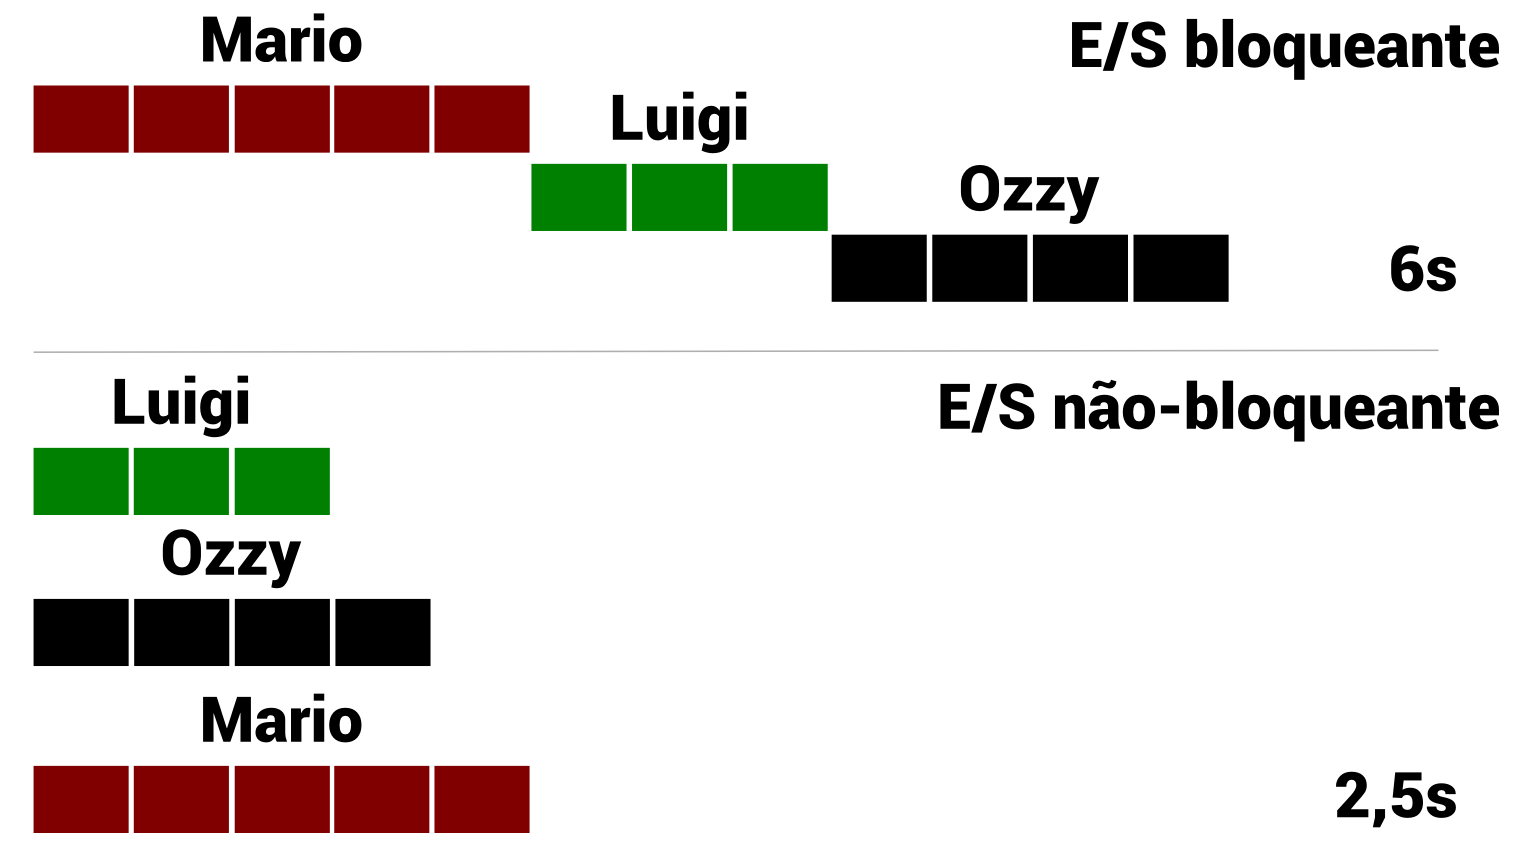
\includegraphics[scale=0.35]{img/throughput.png}

Veja a diferença na vazão.

\end{frame}

\begin{frame}\frametitle{}

\slidetitle{E/S}

\end{frame}

\section{E/S}

\subsection{Operações com arquivos}

\begin{frame}[fragile]\frametitle{Operações com arquivos}

\inputjscodefile{ src/fs1.js }

Este trecho de código eventualmente irá funcionar como esperado. Isso se
fosse uma operação bloqueante, onde o método \texttt{fs.unlink} iria
esperar o método \texttt{fs.readFile}.

\end{frame}

\begin{frame}\frametitle{Operações com arquivos}

Entretanto, estes métodos são assíncronos e podem não funcionar como
esperado.

Então como fazer para resolver isso? Utilize chamadas aninhadas.

\inputjscodefile{ src/fs2.js }

\end{frame}

\begin{frame}[fragile]\frametitle{Operações com arquivos}

Outra opção é utilizar chamadas síncronas do mesmo método.

\inputjscodefile{ src/fs3.js }

\url{http://nodejs.org/api/fs.html}

\end{frame}
